\markdownRendererHeadingFour{Resultados}\markdownRendererInterblockSeparator
{}Al evaluar los resultados añadiendo mayor proporción de agentes que siguen la estrategia Moving Average (MA) se observa que el comportamiento de la serie de tiempo de precios adquiere periodicidad hasta llegar a un punto crítico entre 75% y 80% de agentes MA en donde la simulación converge a un precio estacionario.\markdownRendererInterblockSeparator
{}\begin{figure}[h!] \centering 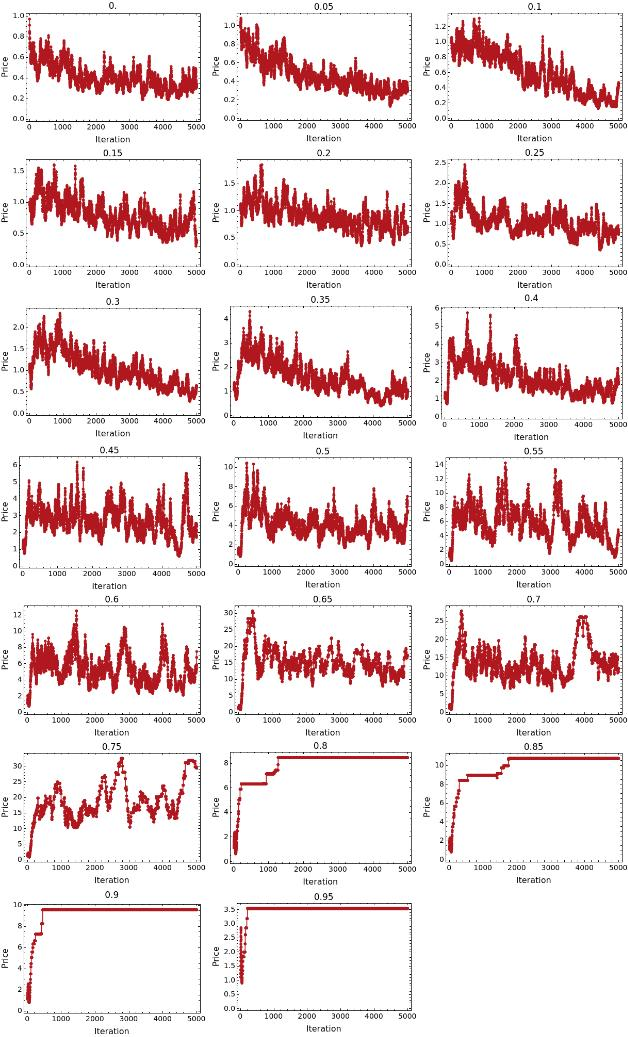
\includegraphics[scale=0.4]{img/price_series.jpeg} \caption{Ejemplo de DAG. Nótese que no existe ninguna secuencia de transiciones que comenzando desde un estado (por ejemplo el $b$), nos regrese al mismo.} \end{figure}\markdownRendererInterblockSeparator
{}\markdownRendererHorizontalRule{}\markdownRendererInterblockSeparator
{}\markdownRendererHeadingFour{This is another sample}\markdownRendererInterblockSeparator
{}\markdownRendererUlBegin
\markdownRendererUlItem Some maths material\markdownRendererUlItemEnd 
\markdownRendererUlEnd \markdownRendererInterblockSeparator
{}\begin{align} A &= U \times S \times V^T\ \sigma &= \frac{x\times y}{\sqrt[3]{\alpha + \beta}} \end{align}\markdownRendererInterblockSeparator
{}\markdownRendererHorizontalRule{}\markdownRendererInterblockSeparator
{}\markdownRendererHeadingFour{\markdownRendererCodeSpan{pipeTables} and \markdownRendererCodeSpan{tableCaptions}}\markdownRendererInterblockSeparator
{}\markdownRendererTable{Demonstration of pipe table syntax.}{4}{4}{rldc}%
{{Right}%
{Left}%
{Default}%
{Center}%
}%
{{12}%
{12}%
{12}%
{12}%
}%
{{123}%
{123}%
{123}%
{123}%
}%
{{1}%
{1}%
{1}%
{1}%
}%
\markdownRendererInterblockSeparator
{}\markdownRendererHorizontalRule{}\relax